\documentclass[11pt,a4paper]{article}

% ---------------------------------------------------------------
% Packages
% ---------------------------------------------------------------
\usepackage[utf8]{inputenc}
\usepackage[T1]{fontenc}
\usepackage{lmodern}
\usepackage[margin=1in]{geometry}
\usepackage{amsmath, amssymb, amsthm, mathtools}
\usepackage{graphicx}
\usepackage{booktabs}
\usepackage{multirow}
\usepackage{array}
\usepackage[expansion=false]{microtype}
\usepackage{listings}
\usepackage{xcolor}
\usepackage{textcomp}
\usepackage{enumitem}
\usepackage{tabularx}
\usepackage{hyperref}
\hypersetup{colorlinks=true, linkcolor=blue!50!black, citecolor=blue!50!black, urlcolor=blue!50!black}

\graphicspath{{figures/}}
\setlength{\emergencystretch}{2em}

\lstdefinestyle{pystyle}{
    language=Python,
    basicstyle=\ttfamily\footnotesize,
    keywordstyle=\color{blue},
    commentstyle=\color{gray},
    stringstyle=\color{teal},
    showstringspaces=false,
    breaklines=true,
    frame=single,
    tabsize=4
}

% ---------------------------------------------------------------
% Theorem environments and macros
% ---------------------------------------------------------------
\theoremstyle{plain}
\newtheorem{theorem}{Theorem}[section]
\newtheorem{proposition}[theorem]{Proposition}
\newtheorem{lemma}[theorem]{Lemma}
\theoremstyle{definition}
\newtheorem{definition}[theorem]{Definition}
\newtheorem{remark}[theorem]{Remark}

\newcommand{\dd}{\mathrm{d}}
\newcommand{\E}{\mathbb{E}}
\newcommand{\Q}{\mathbb{Q}}
\newcommand{\R}{\mathbb{R}}
\newcommand{\bp}{\,\mathrm{bp}}
\newcommand{\eur}{\text{\texteuro}}
\DeclareMathOperator*{\argmin}{arg\,min}

\title{\textbf{Yield Curve Construction:\\
Interpolation, Bootstrapping and Curve Risk}}
\author{\textbf{Elias Benguedda}}
\date{October 2026}

\begin{document}

\maketitle

\begin{abstract}
This paper studies the construction of a zero-coupon yield curve, the first input of every pricing model. We express all interpolation schemes through the integrated forward $y(T)=-\ln P(0,T)$ and compare seven of them on the EURIBOR 6M zero-coupon curve of 12 February 2025: raw (log-linear discount factors), linear and natural cubic spline on zero rates, PCHIP, the monotone convex method of Hagan and West, and the parametric Nelson--Siegel and Svensson curves. The methods are almost indistinguishable on zero rates but very different on the instantaneous forward curve: steps, saw-tooth, overshooting, or a continuous and local curve for monotone convex.

We then bootstrap curves from market instruments (deposits, FRA, swaps, par bonds) with a sequential solver for the raw method and a simultaneous Newton-type solver for the non-local methods. All exact methods reprice the instruments to machine precision, but a round trip on 9 quotes recovers the reference zero rates only within $0.8$--$3\bp$, and on real US Treasury par yields the 30-year forward differs by almost $90\bp$ across methods. A principal component analysis of 181 bootstrapped Treasury curves recovers the level, slope and curvature factors ($79.6\%$, $13.2\%$ and $2.7\%$ of the variance). Finally, key-rate sensitivities of an off-pillar zero-coupon bond show that the interpolation decides which instruments hedge the position, and that monotone convex is strongly non-linear in its inputs: its key rates add up to $-378\,\eur$ for a parallel sensitivity of $-316\,\eur$. This paper is linked to my GitHub, which can be found on my portfolio\footnote{\url{https://portfolio-eliasbenguedda.fr}}, and all scripts are available in the same repository.
\end{abstract}

\clearpage

\tableofcontents
\newpage

% ===============================================================
\section{Introduction}
\label{sec:intro}
% ===============================================================

\subsection{Motivation}
Every pricing model needs a discount curve. In the Heston and local-stochastic volatility papers of this portfolio, the EURIBOR 6M curve enters through the discount factor $D(T)$ and the forward $F(T)$ of the underlying; in rate models such as Hull--White, the whole initial term structure $T\mapsto P(0,T)$ is an input that the model must reproduce exactly. The market, however, only quotes a finite number of instruments (deposits, FRAs, futures, swaps, bonds). Building a curve therefore means solving two problems:
\begin{enumerate}[label=(\roman*)]
    \item an \emph{interpolation} problem: how to define $P(0,T)$ between and beyond the quoted maturities;
    \item an \emph{inverse} problem, the \emph{bootstrap}: how to find the curve whose implied quotes equal the market quotes.
\end{enumerate}
The two problems are not independent: with a non-local interpolation, a new instrument changes the curve before the previous ones, and the bootstrap must be solved globally.

The choice of the interpolation looks like a technical detail, because all the exact methods reproduce the quoted instruments. We show that it is not: the curve between the pillars, the instantaneous forward curve and, above all, the hedge of a cash flow that does not fall on a pillar depend on it. The forward curve is the relevant object, since it drives the floating coupons, the short-rate drift of Hull--White and the long-dated exotics.

\subsection{Organization of the paper}
Section~\ref{sec:prelim} fixes notation and recalls the relations between discount factors, zero rates and forwards. Section~\ref{sec:data} describes the data. Section~\ref{sec:interp} presents the interpolation methods and Section~\ref{sec:comparison} compares them on the EURIBOR curve. Section~\ref{sec:bootstrap} presents the bootstrap and applies it to synthetic and real quotes. Section~\ref{sec:pca} decomposes the daily moves of the Treasury curve in principal components. Section~\ref{sec:risk} studies the key-rate risk of an off-pillar cash flow. Section~\ref{sec:downstream} shows how the curve is used by the pricing models. Section~\ref{sec:limits} discusses the limitations, Section~\ref{sec:next-steps} lists next steps and Section~\ref{sec:conclusion} concludes. Appendix~\ref{app:code} gives excerpts of the Python implementation and Appendix~\ref{app:notation} the notation.

\clearpage
% ===============================================================
\section{Preliminaries and Notation}
\label{sec:prelim}
% ===============================================================

\subsection{Discount factors, zero rates and compounding}
Let $P(0,T)$ be the price today of a zero-coupon bond paying one unit at time $T$, measured in years. Everything in this paper is derived from the \emph{integrated forward}
\begin{equation}
    y(T) = -\ln P(0,T), \qquad y(0)=0.
    \label{eq:y}
\end{equation}
The continuously compounded zero rate is $r(T)=y(T)/T$, so that $P(0,T)=e^{-r(T)T}$. A rate $R$ quoted with another compounding convention is converted with
\begin{equation}
    \text{simple: } 1+R\,T=e^{r(T)T}, \qquad
    \text{$m$ times a year: } \Bigl(1+\frac{R}{m}\Bigr)^{m}=e^{r(T)},
    \label{eq:compounding}
\end{equation}
that is $r=\ln(1+RT)/T$ and $r=m\ln(1+R/m)$ respectively (functions \texttt{to\_continuous} and \texttt{from\_continuous} of \texttt{yield\_curve.py}).

\subsection{Forward rates}
The forward rate between $T_1<T_2$ seen today is the rate that can be locked today for a loan over $[T_1,T_2]$:
\begin{equation}
    f(0;T_1,T_2)=\frac{y(T_2)-y(T_1)}{T_2-T_1}\ \text{(continuous)}, \qquad
    F(0;T_1,T_2)=\frac{1}{T_2-T_1}\Bigl(\frac{P(0,T_1)}{P(0,T_2)}-1\Bigr)\ \text{(simple)}.
    \label{eq:fwd}
\end{equation}
The simple forward is the fair rate of a FRA and, in a single-curve framework, the expected value of the floating fixing under the $T_2$-forward measure. Letting $T_2\to T_1=T$ gives the \emph{instantaneous forward rate}
\begin{equation}
    f(0,T)=-\frac{\partial\ln P(0,T)}{\partial T}=y'(T)=r(T)+T\,r'(T),
    \qquad
    P(0,T)=\exp\Bigl(-\int_0^Tf(0,s)\,\dd s\Bigr).
    \label{eq:instfwd}
\end{equation}
The relation $f=r+Tr'$ is the reason why the forward curve is a much more sensitive diagnostic than the zero curve: it involves the \emph{derivative} of the zero rates, multiplied by the maturity. A kink of the zero curve becomes a jump of the forward, and a small oscillation of $r$ at $T=20$ years is amplified twenty times.

\subsection{Discrete forwards: what the data contain}
Given pillars $0=t_0<t_1<\dots<t_n$ with zero rates $r_i=r(t_i)$, the \emph{discrete forwards}
\begin{equation}
    f^d_i=\frac{r_it_i-r_{i-1}t_{i-1}}{t_i-t_{i-1}}=\frac{1}{t_i-t_{i-1}}\int_{t_{i-1}}^{t_i}f(0,s)\,\dd s, \qquad i=1,\dots,n,
    \label{eq:discrete-fwd}
\end{equation}
are the only forward information contained in the data. By~\eqref{eq:instfwd}, an interpolation passes through all the pillars if and only if its instantaneous forward has average $f^d_i$ on each segment $(t_{i-1},t_i]$. Everything else (the shape of $f$ inside a segment, its continuity at the pillars) is a modelling choice.

\begin{remark}[A mean-value constraint]\label{rem:mean}
If an exact interpolation has a continuous forward curve and $f(0,t_{i-1})<f^d_i$ and $f(0,t_i)<f^d_i$, then $f$ must exceed $f^d_i$ somewhere inside the segment, since its average is $f^d_i$. This simple observation explains the forward humps of Section~\ref{sec:treasury}.
\end{remark}

\subsection{Annuity and par rates}
For a fixed leg paying at $t_1<\dots<t_N=T$ with accrual fractions $\delta_j=t_j-t_{j-1}$, the annuity (PV01 of a unit notional) is
\begin{equation}
    A(T)=\sum_{j=1}^{N}\delta_j\,P(0,t_j).
    \label{eq:annuity}
\end{equation}
In a single-curve framework the floating leg of a swap starting today is worth $1-P(0,T)$ (telescoping sum of the forward fixings~\eqref{eq:fwd}), so the par swap rate, which is also the par yield of a bond, is
\begin{equation}
    S(T)=\frac{1-P(0,T)}{A(T)}.
    \label{eq:par}
\end{equation}

\subsection{Notation}
Table~\ref{tab:notation} in Appendix~\ref{app:notation} summarizes the notation used throughout the paper.

\clearpage
% ===============================================================
\section{Data}
\label{sec:data}
% ===============================================================

\subsection{EURIBOR 6M zero-coupon curve}
The first data set is the EURIBOR 6M zero-coupon curve of 12 February 2025 already used for the Heston calibration~\cite{data}. It is given at 15 pillars from 1 week ($t_1=0.02$) to 5 years, with rates rounded to the basis point. The rates are taken as continuously compounded. Table~\ref{tab:euribor} gives the zero rates and the discrete forwards~\eqref{eq:discrete-fwd}.

\begin{table}[htbp]
\centering
\small
\begin{tabular}{@{}lrrrrrrrr@{}}
\toprule
Maturity (y) & 0.02 & 0.25 & 0.50 & 0.75 & 1.00 & 1.25 & 1.50 & 1.75 \\
Zero rate (\%) & 2.68 & 2.64 & 2.51 & 2.39 & 2.33 & 2.28 & 2.26 & 2.25 \\
Discrete forward (\%) & 2.68 & 2.637 & 2.38 & 2.15 & 2.15 & 2.08 & 2.16 & 2.19 \\
\midrule
Maturity (y) & 2.00 & 2.50 & 3.00 & 3.50 & 4.00 & 4.50 & 5.00 & \\
Zero rate (\%) & 2.24 & 2.25 & 2.26 & 2.27 & 2.28 & 2.29 & 2.30 & \\
Discrete forward (\%) & 2.17 & 2.29 & 2.31 & 2.33 & 2.35 & 2.37 & 2.39 & \\
\bottomrule
\end{tabular}
\caption{EURIBOR 6M zero-coupon rates (12/02/2025) and discrete forwards on each segment $(t_{i-1},t_i]$.}
\label{tab:euribor}
\end{table}

The zero curve is inverted up to two years, reflecting the expected ECB rate cuts, then slightly upward sloping (Figure~\ref{fig:euribor}). The discrete forwards are much more irregular than the zero rates: they move by $23\bp$ between the $0.25$--$0.5$ and $0.5$--$0.75$ segments, and from $2.17\%$ to $2.29\%$ at two years. Since a forward is a discrete derivative of $r(T)T$, the rounding of the data to $\pm0.5\bp$ becomes an error of up to $\frac12\bp\times(t_i+t_{i-1})/(t_i-t_{i-1})$ on $f^d_i$, i.e. $7.5\bp$ on the $1.75$--$2$ year segment and $9.5\bp$ on the $4.5$--$5$ year segment. This is the first reason why interpolations must be judged on the forward curve.

\begin{figure}[htbp]
    \centering
    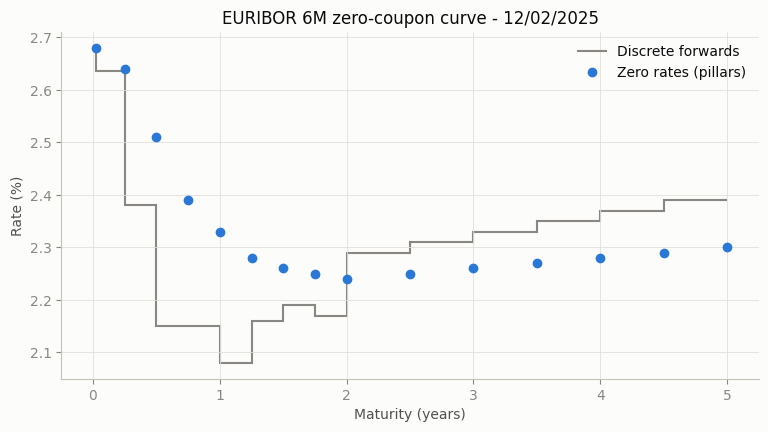
\includegraphics[width=0.75\textwidth]{euribor_data.png}
    \caption{EURIBOR 6M zero rates at the pillars and discrete forwards (step function).}
    \label{fig:euribor}
\end{figure}

\subsection{US Treasury par yield curve}
The second data set is the daily US Treasury par yield curve~\cite{treasury} from 2 January to 21 September 2026 (181 dates), with 14 tenors: bills of 1, 1.5, 2, 3, 4 and 6 months and 1 year, then coupon securities of 2, 3, 5, 7, 10, 20 and 30 years. These are real market quotes, and the long end is sparse (7, 10, 20, 30 years), which makes them a good test of the interpolation between distant pillars. We use the following simplified conventions:
\begin{itemize}
    \item bills up to 6 months are treated as simple-rate zero-coupons, $1+RT=1/P(0,T)$;
    \item the 1-year bill as a semi-annually compounded zero-coupon (bond-equivalent yield);
    \item notes and bonds as semi-annual par bonds, priced by~\eqref{eq:par} with $\delta_j=\frac12$.
\end{itemize}
No day-count convention, calendar or settlement lag is applied (Section~\ref{sec:limits}).

\clearpage
% ===============================================================
\section{Interpolation Methods}
\label{sec:interp}
% ===============================================================

\subsection{A common framework}
All the methods are implemented in \texttt{interpolation.py} as subclasses of \texttt{CurveInterpolator}, built on the pillars $(t_i,r_i)$ and exposing three functions: $y(T)$, $r(T)$ and $f(0,T)=y'(T)$. Discount factors are always computed as $e^{-y(T)}$ and forwards as differences of $y$, so that the three quantities are exactly consistent. Two conventions are shared by the exact methods:
\begin{itemize}
    \item \textbf{before the first pillar} the zero rate is flat, $y(T)=r_1T$, i.e. a constant forward $r_1$ on $[0,t_1]$ (except for the raw and monotone convex methods, which define the curve on $[0,t_1]$ themselves with the origin $y(0)=0$ as an additional node);
    \item \textbf{after the last pillar} the instantaneous forward is flat, $y(T)=y(t_n)+f(0,t_n)(T-t_n)$, which avoids the explosion of the forward that a flat zero-rate extrapolation would cause by~\eqref{eq:instfwd}.
\end{itemize}
A method is \emph{exact} if it passes through every pillar, and \emph{local} if moving one pillar only changes the curve on the neighbouring segments. Locality matters for hedging: with a non-local method, a move of the 2-year rate changes the value of a 4-year cash flow, which is then hedged with 2-year instruments.

\subsection{Raw interpolation (log-linear discount factors)}
The market-standard "raw" method interpolates $y$ linearly between the nodes $t_0=0,t_1,\dots,t_n$:
\begin{equation}
    y(T)=y(t_{i-1})+f^d_i\,(T-t_{i-1}),\qquad f(0,T)=f^d_i\quad\text{on }(t_{i-1},t_i].
\end{equation}
The forward curve is piecewise constant and equal to the discrete forwards. The method is perfectly local, linear in the pillar values $y_i$, and produces positive forwards whenever the discrete forwards are positive. Its drawback is the step-shaped forward curve: a FRA straddling a pillar is priced with two unrelated forwards.

\subsection{Linear interpolation of the zero rates}
The zero rate is linear on each segment, $r(T)=r_{i-1}+s_i(T-t_{i-1})$ with $s_i=(r_i-r_{i-1})/(t_i-t_{i-1})$. By~\eqref{eq:instfwd}, $f(0,T)=r(T)+Ts_i$, which is linear but discontinuous at each pillar with jump
\begin{equation}
    f(0,t_i^+)-f(0,t_i^-)=t_i\,(s_{i+1}-s_i).
\end{equation}
The jump grows with the maturity: the forward curve has a saw-tooth shape.

\subsection{Natural cubic spline on the zero rates}
$r(T)$ is the natural cubic spline through the pillars ($C^2$, with $r''=0$ at both ends), computed by \texttt{scipy.interpolate.CubicSpline}. The forward $f=r+Tr'$ is then $C^1$. The spline coefficients solve a tridiagonal linear system whose inverse is a full matrix: the method is \emph{linear} in the data but \emph{non-local}, every pillar moving the whole curve with alternating-sign oscillations that decay geometrically away from it. The forward also overshoots the discrete forwards where the data turn sharply.

\subsection{PCHIP on the zero rates}
The Piecewise Cubic Hermite Interpolating Polynomial of Fritsch and Carlson~\cite{fritsch} is a $C^1$ cubic on each segment, whose derivatives at the nodes are chosen to preserve monotonicity. With $\Delta_i=s_i$ the slopes of the data and $h_i=t_i-t_{i-1}$, the derivative at an inner node is zero if $\Delta_i\Delta_{i+1}\le0$ and otherwise the weighted harmonic mean
\begin{equation}
    \frac{w_1+w_2}{r'(t_i)}=\frac{w_1}{\Delta_i}+\frac{w_2}{\Delta_{i+1}},\qquad w_1=2h_{i+1}+h_i,\quad w_2=h_{i+1}+2h_i.
\end{equation}
The zero rates never overshoot the data and the method is almost local (the curve on a segment depends on four neighbouring pillars). But the forward $f=r+Tr'$ is only continuous, and its shape is not controlled: PCHIP controls the zero rates, not the forwards. The harmonic mean also makes the method \emph{non-linear} in the data, which matters for risk (Section~\ref{sec:risk}).

\subsection{The monotone convex method}
\label{sec:mc}
The monotone convex method of Hagan and West~\cite{haganwest2006, haganwest2008} interpolates the instantaneous forward curve directly. It is the default method of the \texttt{YieldCurve} class.

\paragraph{Node forwards.} With the origin as a node ($\tau_0=0,\tau_i=t_i$), the instantaneous forwards at the nodes are weighted averages of the neighbouring discrete forwards,
\begin{equation}
    f_i=\frac{\tau_i-\tau_{i-1}}{\tau_{i+1}-\tau_{i-1}}\,f^d_{i+1}+\frac{\tau_{i+1}-\tau_i}{\tau_{i+1}-\tau_{i-1}}\,f^d_i,\qquad i=1,\dots,n-1,
\end{equation}
and at the end points $f_0=f^d_1-\tfrac12(f_1-f^d_1)$, $f_n=f^d_n-\tfrac12(f_{n-1}-f^d_n)$.

\paragraph{Correction function.} On the segment $(\tau_{i-1},\tau_i]$, with $x=(T-\tau_{i-1})/(\tau_i-\tau_{i-1})\in[0,1]$, the forward is written
\begin{equation}
    f(0,T)=f^d_i+g(x),\qquad g(0)=g_0:=f_{i-1}-f^d_i,\quad g(1)=g_1:=f_i-f^d_i,\quad \int_0^1g(x)\,\dd x=0.
    \label{eq:mc-g}
\end{equation}
The last condition guarantees that the forward averages to $f^d_i$ on the segment, hence the exactness. The function $g$ is chosen according to the signs of $(g_0,g_1)$, so that $f$ stays monotone where the data are monotone (Table~\ref{tab:mc-regions}).

\begin{table}[htbp]
\centering
\small
\renewcommand{\arraystretch}{1.35}
\begin{tabular}{@{}p{3.2cm}p{4.2cm}p{7.3cm}@{}}
\toprule
Region & Condition & Correction $g(x)$ \\
\midrule
(i) cubic & $g_1$ between $-2g_0$ and $-\tfrac12g_0$ & $g_0(1-4x+3x^2)+g_1(-2x+3x^2)$ \\
(ii) flat then quadratic & $g_0<0,\ g_1>-2g_0$ (or symmetric) & $g_0$ on $[0,\eta]$, then $g_0+(g_1-g_0)\bigl(\frac{x-\eta}{1-\eta}\bigr)^2$, \ $\eta=\frac{g_1+2g_0}{g_1-g_0}$ \\
(iii) quadratic then flat & $g_0>0,\ -\tfrac12g_0<g_1<0$ (or symmetric) & $g_1+(g_0-g_1)\bigl(\frac{\eta-x}{\eta}\bigr)^2$ on $[0,\eta]$, then $g_1$, \ $\eta=\frac{3g_1}{g_1-g_0}$ \\
(iv) two quadratics & $g_0,g_1$ of the same sign & $A+(g_0-A)\bigl(\frac{\eta-x}{\eta}\bigr)^2$ on $[0,\eta]$, then $A+(g_1-A)\bigl(\frac{x-\eta}{1-\eta}\bigr)^2$, \ $\eta=\frac{g_1}{g_0+g_1}$, $A=-\frac{g_0g_1}{g_0+g_1}$ \\
\bottomrule
\end{tabular}
\caption{The four regions of the monotone convex method. In region (i) the cubic is the unique quadratic-in-$x$ correction with zero mean; outside it, the cubic would overshoot and is replaced by piecewise quadratics with a flat part.}
\label{tab:mc-regions}
\end{table}

The integrated forward is obtained in closed form from the primitive $G(x)=\int_0^xg$:
\begin{equation}
    y(T)=y(\tau_{i-1})+f^d_i\,(T-\tau_{i-1})+(\tau_i-\tau_{i-1})\,G(x).
\end{equation}
The resulting forward curve is continuous, reproduces the discrete forwards exactly, stays within the range of the neighbouring discrete forwards, and is local: a pillar only moves the node forwards $f_{i-1},f_i$ and therefore the curve on the two or three neighbouring segments.

\paragraph{Implementation details.} Two points required care. (a) The formulas are vectorized with masks over the four regions. (b) With rates rounded to the basis point, two consecutive discrete forwards are frequently equal, so that exactly one of $g_0,g_1$ vanishes: regions (iii) and (iv) then degenerate into a jump ($\eta\in\{0,1\}$). In that case the cubic of region (i) is used, which is continuous and exact. Values of $|g|<10^{-12}$ are set to zero to absorb round-off. The positivity "collar" of Hagan and West, which bounds the node forwards to keep $f\ge0$, is not implemented since all forwards are positive here.

\subsection{Parametric curves: Nelson--Siegel and Svensson}
Nelson and Siegel~\cite{nelsonsiegel} and Svensson~\cite{svensson} describe the whole curve with a few interpretable parameters. With $x_k=T/\lambda_k$,
\begin{equation}
    r(T)=\beta_0+\beta_1\frac{1-e^{-x_1}}{x_1}+\beta_2\Bigl(\frac{1-e^{-x_1}}{x_1}-e^{-x_1}\Bigr)+\beta_3\Bigl(\frac{1-e^{-x_2}}{x_2}-e^{-x_2}\Bigr),
    \label{eq:ns}
\end{equation}
with $\beta_3=0$ for Nelson--Siegel (4 parameters) and 6 parameters for Svensson. Here $\lambda_k$ is a time scale in years. The forward curve has the simpler form
\begin{equation}
    f(0,T)=\beta_0+\beta_1e^{-x_1}+\beta_2x_1e^{-x_1}+\beta_3x_2e^{-x_2},
\end{equation}
so that $r(0)=f(0,0)=\beta_0+\beta_1$ and $r(\infty)=\beta_0$: $\beta_0$ is the level, $\beta_1$ minus the slope, $\beta_2,\beta_3$ the curvatures (humps located around $T\approx\lambda_k$).

\paragraph{Fitting.} The curves are fitted by least squares on the zero rates at the pillars. Given the $\lambda$'s, the model~\eqref{eq:ns} is linear in the $\beta$'s, which are obtained by ordinary least squares; the problem is thus reduced to the $\lambda$'s only (variable projection). For Nelson--Siegel, $\lambda_1$ is first located on a grid of 200 values in $[0.05,10]$, then refined by a bounded Brent search~\cite{brent} on $[\lambda^\star/2,2\lambda^\star]$. For Svensson, a $25\times25$ grid with $\lambda_2>1.2\lambda_1$ (to separate the two humps) provides the starting point of a Nelder--Mead search. The parametric curves are defined for all $T\ge0$ without extrapolation rule, but they do \emph{not} reprice the inputs: they are used by central banks and for smoothing or factor models, not for pricing, and they cannot be bootstrapped.

\subsection{Summary}
\begin{table}[htbp]
\centering
\small
\begin{tabular}{@{}lllcc@{}}
\toprule
Method & Interpolated quantity & Forward curve & Local & Exact \\
\midrule
Raw & $y=-\ln P$ linear & piecewise constant (steps) & yes & yes \\
Linear zero & $r$ linear & discontinuous (saw-tooth) & yes & yes \\
Cubic spline zero & $r$ natural cubic spline & $C^1$ & no & yes \\
PCHIP zero & $r$ monotone cubic Hermite & $C^0$, not controlled & almost & yes \\
Monotone convex & $f$ (Hagan--West) & $C^0$, no spurious oscillation & almost & yes \\
Nelson--Siegel & parametric, 4 parameters & smooth & no & no \\
Svensson & parametric, 6 parameters & smooth & no & no \\
\bottomrule
\end{tabular}
\caption{The seven interpolation methods implemented in \texttt{interpolation.py}.}
\label{tab:methods}
\end{table}

\clearpage
% ===============================================================
\section{Comparison on the EURIBOR Curve}
\label{sec:comparison}
% ===============================================================

\subsection{Zero and forward curves}
On the zero rates (Figure~\ref{fig:zero}) the exact methods are almost indistinguishable: they all go through the pillars and differ by a fraction of a basis point in between. The parametric curves miss the pillars, Nelson--Siegel by up to $5\bp$ at the short end. The forward curves (Figure~\ref{fig:forwards}) reveal the differences:
\begin{itemize}
    \item \textbf{raw}: the forward is exactly the discrete forward, a step function;
    \item \textbf{linear zero}: saw-tooth forwards, with a jump at every pillar (up to $18\bp$);
    \item \textbf{cubic spline and PCHIP}: smooth zero rates, but the forward $f=r+Tr'$ overshoots the discrete forwards, with dips below $2.07\%$ around one year;
    \item \textbf{monotone convex}: continuous forward which stays within the range of the neighbouring discrete forwards;
    \item \textbf{Nelson--Siegel and Svensson}: very smooth, but they average the data instead of reproducing it; Nelson--Siegel misses the inversion and rises to $2.5\%$ at $5.5$ years, $11\bp$ above the last discrete forward.
\end{itemize}

\begin{figure}[htbp]
    \centering
    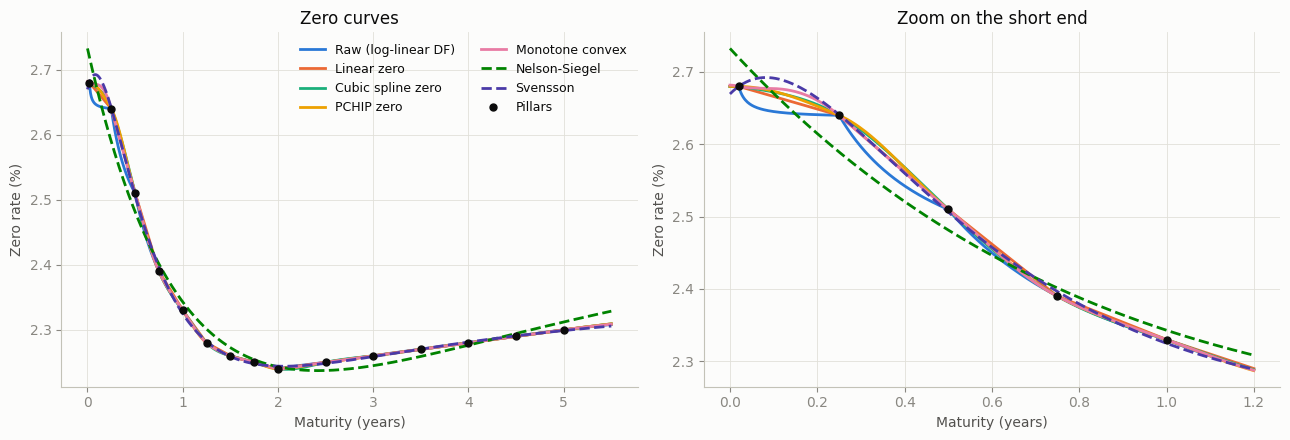
\includegraphics[width=\textwidth]{zero_curves.png}
    \caption{Zero curves of the seven methods (left) and zoom on the short end (right).}
    \label{fig:zero}
\end{figure}

\begin{figure}[htbp]
    \centering
    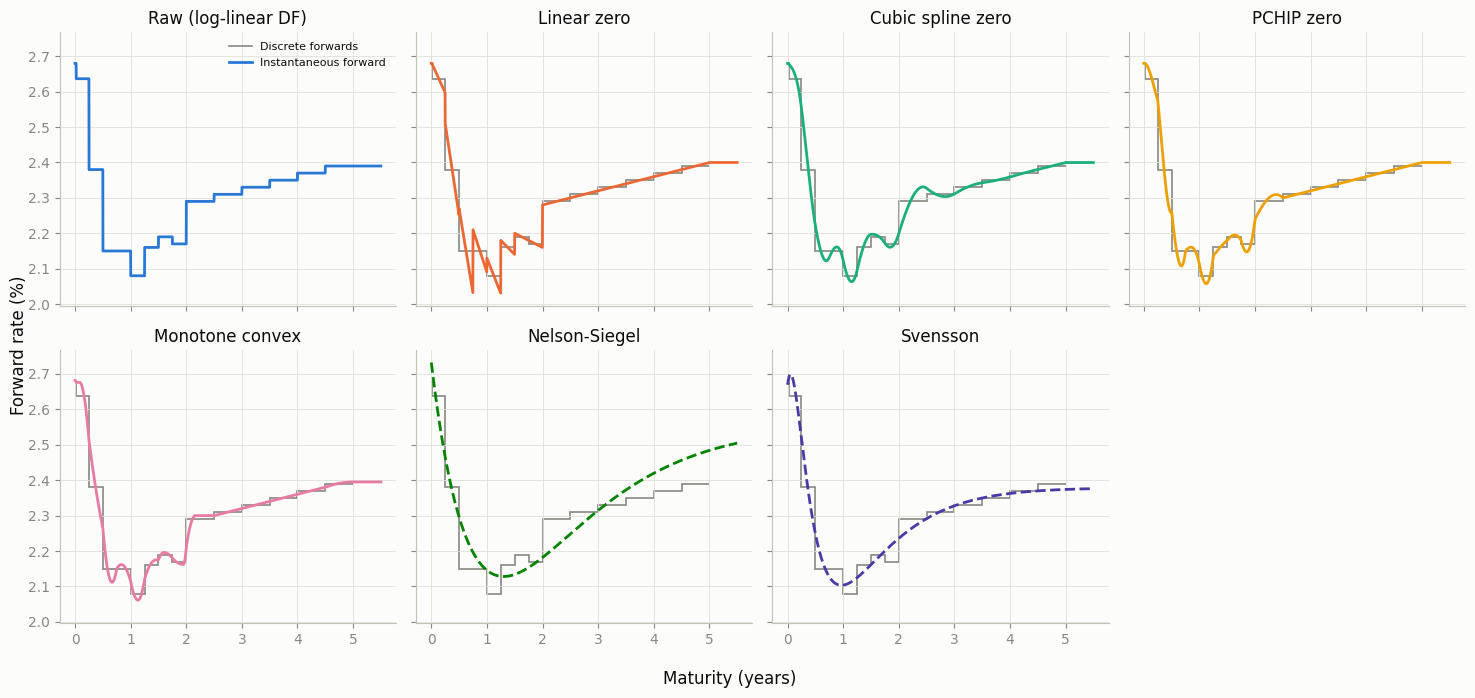
\includegraphics[width=\textwidth]{forward_curves.png}
    \caption{Instantaneous forward curves of the seven methods against the discrete forwards (grey steps).}
    \label{fig:forwards}
\end{figure}

\subsection{Quantitative comparison}
We measure, on a grid of 5001 points on $[0,5]$:
\begin{itemize}
    \item the \emph{pillar error}, largest gap between the curve and the input zero rates;
    \item the \emph{forward jump}, largest discontinuity of $f$ at an inner pillar;
    \item the \emph{forward total variation} $\sum|\Delta f|$, a measure of how much the forward curve oscillates; the discrete forwards themselves give the reference value of $95.0\bp$;
    \item the \emph{locality}: the 2-year zero rate is bumped by $+1\bp$, and we report the largest forward change, everywhere and far from the bump (outside $[1.5,3]$ years);
    \item the evaluation time per point of the discount factor.
\end{itemize}

\begin{table}[htbp]
\centering
\small
\begin{tabular}{@{}lrrrrrrr@{}}
\toprule
& Pillar & Max fwd & Fwd total & Fwd min & Fwd max & \multicolumn{2}{c}{2y bump: max $|\Delta f|$} \\
\cmidrule(l){7-8}
Method & error (bp) & jump (bp) & var. (bp) & (\%) & (\%) & all (bp) & far (bp) \\
\midrule
Raw & 0.000 & 25.65 & 95.0 & 2.080 & 2.680 & 8.00 & 0.00 \\
Linear zero & 0.000 & 18.00 & 165.4 & 2.030 & 2.680 & 8.99 & 0.00 \\
Cubic spline zero & 0.000 & 0.00 & 115.9 & 2.063 & 2.680 & 9.46 & 1.83 \\
PCHIP zero & 0.000 & 0.00 & 118.7 & 2.058 & 2.680 & 10.27 & 0.00 \\
Monotone convex & 0.000 & 0.00 & 112.2 & 2.061 & 2.682 & 9.76 & 0.00 \\
Nelson--Siegel & 5.072 & 0.00 & 96.0 & 2.128 & 2.732 & 0.74 & 0.74 \\
Svensson & 0.648 & 0.00 & 89.6 & 2.103 & 2.699 & 0.65 & 0.65 \\
\bottomrule
\end{tabular}
\caption{Comparison of the interpolation methods on the EURIBOR 6M curve. "Far" means outside $[1.5,3]$ years. Evaluation times range from $0.016\,\mu$s per point (raw) to $0.17\,\mu$s (monotone convex).}
\label{tab:comparison}
\end{table}

Among the exact methods, raw has the lowest forward total variation, which is the variation of the data itself, but a step forward. Monotone convex has the lowest variation of the continuous methods ($112\bp$ against $116$ for the cubic spline, $119$ for PCHIP and $165$ for linear zero). All exact methods move the forward by $8$ to $10\bp$ near the bump, which is the expected order: a $1\bp$ move of $r(2)$ changes $y(2)$ by $2\bp$, hence the discrete forwards of the two neighbouring segments by $2\bp/0.25=8\bp$ and $2\bp/0.5=4\bp$.

\subsection{Locality}
Figure~\ref{fig:bump} shows the response of the forward curve to the $+1\bp$ bump of the 2-year zero rate. Raw, linear zero, PCHIP and monotone convex keep the bump within $[1.5,3]$ years. The natural cubic spline propagates it along the whole curve, with up to $1.8\bp$ of forward change outside that window and alternating signs. The parametric curves spread it everywhere since they refit all their parameters, but with a small amplitude ($<0.75\bp$) since one pillar has little weight in a least-squares fit.

\begin{figure}[htbp]
    \centering
    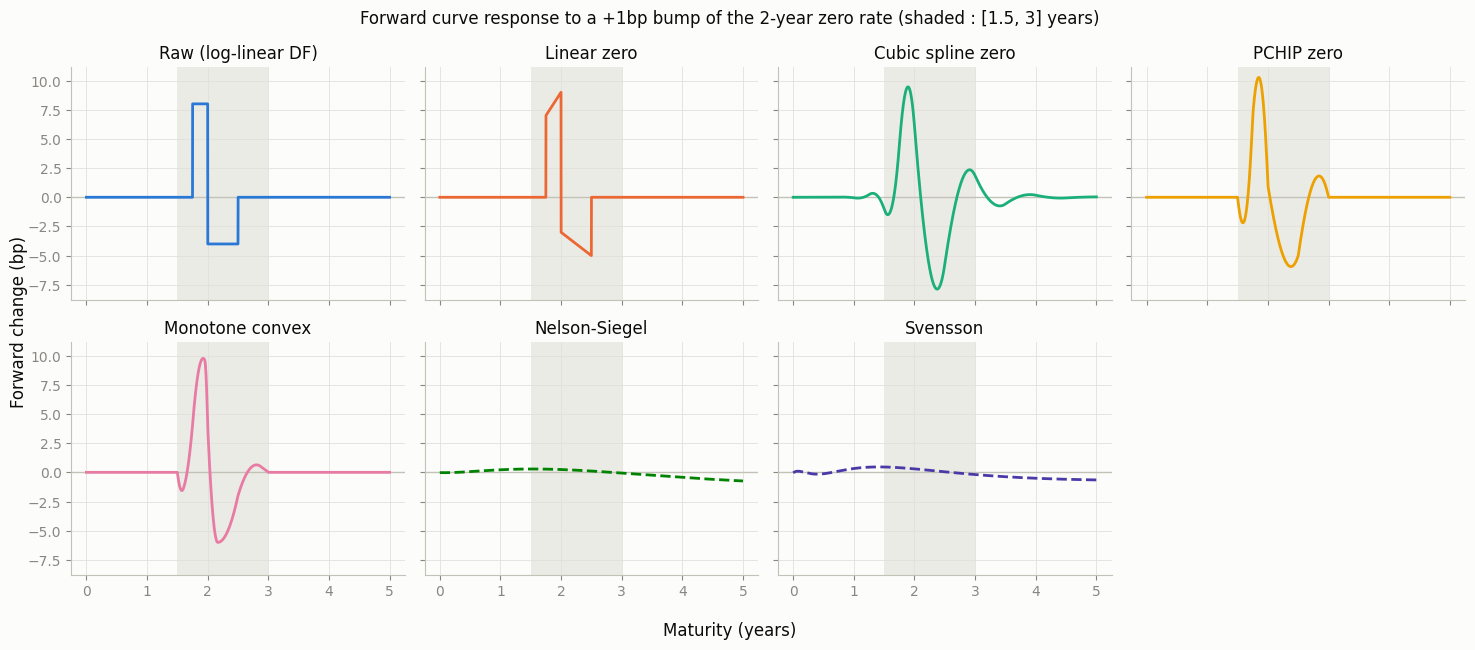
\includegraphics[width=\textwidth]{bump_locality.png}
    \caption{Forward curve response to a $+1\bp$ bump of the 2-year zero rate (shaded: $[1.5,3]$ years).}
    \label{fig:bump}
\end{figure}

Monotone convex is therefore the only method combining exact pillars, a continuous forward curve and locality, which is why it is a market standard~\cite{haganwest2006}.

\subsection{Parametric curves}
Table~\ref{tab:ns} gives the fitted parameters and the residuals at the pillars. Nelson--Siegel has a single hump and cannot reproduce at the same time the sharp inversion of the first year and the slow rise after two years: its residuals reach $-5.1\bp$ at 3 months and $+3.9\bp$ at 1 week, with a clear pattern. The second hump of Svensson, with a short time scale $\lambda_1=0.20$ year, captures the inversion, and the residuals fall below $0.65\bp$, i.e. of the order of the 1bp rounding of the data. Both are good descriptive tools; neither can be used to price instruments that are quoted to a fraction of a basis point.

\begin{table}[htbp]
\centering
\small
\begin{tabular}{@{}lrrrrrr@{}}
\toprule
& $\beta_0$ (\%) & $\beta_1$ (\%) & $\beta_2$ (\%) & $\lambda_1$ (y) & $\beta_3$ (\%) & $\lambda_2$ (y) \\
\midrule
Nelson--Siegel & 2.556 & 0.176 & $-1.329$ & 1.148 & -- & -- \\
Svensson & 2.379 & 0.291 & 0.781 & 0.197 & $-0.883$ & 0.696 \\
\bottomrule
\end{tabular}

\vspace{3mm}
\begin{tabular}{@{}lrrrrrrrr@{}}
\toprule
Residual (bp) & 0.02 & 0.25 & 0.5 & 0.75 & 1 & 1.25 & 1.5 & 1.75 \\
\midrule
Nelson--Siegel & 3.95 & $-5.07$ & $-2.85$ & 1.14 & 1.29 & 2.13 & 1.27 & 0.41 \\
Svensson & $-0.01$ & 0.10 & $-0.37$ & 0.65 & $-0.52$ & 0.23 & $-0.10$ & $-0.22$ \\
\midrule
Residual (bp) & 2 & 2.5 & 3 & 3.5 & 4 & 4.5 & 5 & \\
\midrule
Nelson--Siegel & 0.32 & $-1.25$ & $-1.51$ & $-1.09$ & $-0.37$ & 0.44 & 1.20 & \\
Svensson & 0.41 & $-0.16$ & $-0.12$ & 0.04 & 0.12 & 0.07 & $-0.12$ & \\
\bottomrule
\end{tabular}
\caption{Fitted Nelson--Siegel and Svensson parameters and residuals (model minus market) at the pillars.}
\label{tab:ns}
\end{table}

\clearpage
% ===============================================================
\section{Bootstrapping}
\label{sec:bootstrap}
% ===============================================================

\subsection{Instruments}
In practice the curve is not given as zero rates but implied from quoted instruments. Each instrument of \texttt{instruments.py} knows its market quote $q_k$ and the quote $\hat q_k(\text{curve})$ implied by a curve. We work in a single-curve framework: the same curve discounts the cash flows and projects the floating rates (Table~\ref{tab:instruments}).

\begin{table}[htbp]
\centering
\begin{tabular}{@{}lll@{}}
\toprule
Instrument & Quote & Pricing equation \\
\midrule
Zero-coupon rate & rate $R$, any compounding & conversion~\eqref{eq:compounding} \\
Deposit & simple rate $R$ & $1+R\,T=1/P(0,T)$ \\
FRA $[T_1,T_2]$ & simple forward $R$ & $1+R\,(T_2-T_1)=P(0,T_1)/P(0,T_2)$ \\
Swap / par bond & par rate $S$ & $S\sum_j\delta_jP(0,t_j)=1-P(0,T)$ \\
\bottomrule
\end{tabular}
\caption{Curve instruments and their pricing equations (year fractions, no day count or settlement lag). The fixed-leg schedule runs backwards from the maturity, with a short first period if needed.}
\label{tab:instruments}
\end{table}

\subsection{The bootstrap problem}
One pillar is placed at each instrument maturity $T_k$, and the unknowns are the continuously compounded zero rates $z=(z_1,\dots,z_n)$ at the pillars. The bootstrap solves the square system
\begin{equation}
    R_k(z)=\hat q_k\bigl(\text{curve}(z)\bigr)-q_k=0,\qquad k=1,\dots,n.
    \label{eq:bootstrap}
\end{equation}

\paragraph{Sequential bootstrap (raw interpolation).} An instrument maturing at $T_k$ only depends on $P(0,t)$ for $t\le T_k$. With the raw method, the curve on $[0,T_k]$ only depends on $z_1,\dots,z_k$: the system~\eqref{eq:bootstrap} is \emph{triangular}, and can be solved instrument by instrument, in maturity order, with a one-dimensional root search on $z_k$ (Brent's method~\cite{brent} on $[-50\%,100\%]$, tolerance $10^{-15}$). This is exact.

\paragraph{Simultaneous solve (non-local interpolation).} With a cubic spline, PCHIP or monotone convex, adding the pillar $T_{k+1}$ changes the curve \emph{before} $T_k$ (the spline globally; PCHIP through the slope at $t_k$; monotone convex through the node forward $f_k$, which depends on $f^d_{k+1}$), so the previous instruments are no longer repriced. The $n$ equations are then solved together with the hybrid Powell method of MINPACK~\cite{powell} (\texttt{scipy.optimize.root}, method \texttt{hybr}, finite-difference Jacobian), starting from the raw solution, which is already within a few basis points of the answer. Linear interpolation of the zero rates is local and could be bootstrapped sequentially too; the implementation treats it with the generic simultaneous solver.

\paragraph{Parametric curves.} Nelson--Siegel and Svensson have fewer parameters than instruments and cannot solve~\eqref{eq:bootstrap}. The \texttt{Bootstrapper} refuses them; they must be fitted on the bootstrapped zero rates instead.

After the solve, the maximum residual $\max_k|R_k|$ is checked against a tolerance of $10^{-10}$, i.e. $10^{-6}\bp$, and a warning is printed if it is exceeded. The method \texttt{report()} returns, for each instrument, the market quote, the implied quote, the residual and the zero rate.

\subsection{Round trip on the EURIBOR curve}
To measure what is lost when the curve is built from instruments, we generate market quotes from the monotone convex EURIBOR curve of Section~\ref{sec:comparison} (the \emph{reference}, 15 pillars): 1M, 3M and 6M deposits, a $6\times12$ FRA, a 1.5-year semi-annual swap and 2- to 5-year annual swaps. The curve is then bootstrapped back from these 9 quotes only (Table~\ref{tab:quotes}).

\begin{table}[htbp]
\centering
\footnotesize
\setlength{\tabcolsep}{3pt}
\begin{tabular}{@{}lrrrrrrrrr@{}}
\toprule
Instrument & Dep 1M & Dep 3M & Dep 6M & FRA $6\times12$ & Swap 1.5y & Swap 2y & Swap 3y & Swap 4y & Swap 5y \\
\midrule
Quote (\%) & 2.6803 & 2.6487 & 2.5258 & 2.1616 & 2.2743 & 2.2663 & 2.2860 & 2.3057 & 2.3253 \\
Zero rate (\%) & 2.6774 & 2.6400 & 2.5100 & 2.3300 & 2.2600 & 2.2400 & 2.2600 & 2.2800 & 2.3000 \\
\bottomrule
\end{tabular}
\caption{Synthetic quotes generated from the reference EURIBOR curve and bootstrapped zero rates at the instrument maturities (monotone convex).}
\label{tab:quotes}
\end{table}

\begin{table}[htbp]
\centering
\footnotesize
\begin{tabular}{@{}llrrrr@{}}
\toprule
Method & Solver & Max residual (bp) & Time (ms) & Max $|\Delta r|$ (bp) & Max $|\Delta f|$ (bp) \\
\midrule
Raw & sequential & 0.0 & 7.8 & 2.16 & 13.10 \\
Linear zero & simultaneous (hybr) & 0.0 & 14.0 & 3.04 & 14.48 \\
Cubic spline zero & simultaneous (hybr) & 0.0 & 17.5 & 1.00 & 5.37 \\
PCHIP zero & simultaneous (hybr) & 0.0 & 17.8 & 1.67 & 7.37 \\
Monotone convex & simultaneous (hybr) & 0.0 & 47.4 & 0.83 & 5.84 \\
\bottomrule
\end{tabular}
\caption{Round trip: bootstrap from 9 quotes, and largest gap with the 15-pillar reference curve on the zero rates and on the instantaneous forwards, over $[0.01,5]$ years.}
\label{tab:roundtrip}
\end{table}

Every method reprices the 9 quotes to machine precision (Table~\ref{tab:roundtrip}), yet the curves differ between the pillars: with 9 quotes instead of 15 pillars, the zero rates are recovered within $0.8$ to $3\bp$ and the forwards within $5$ to $14\bp$ (Figure~\ref{fig:roundtrip}). The smallest zero-rate error is obtained by monotone convex, which is also the method that generated the reference: this favours it by construction and should not be over-interpreted. The main lesson is elsewhere: \emph{the interpolation is a modelling assumption}, since the market only pins down the instruments, not what happens in between.

\begin{figure}[htbp]
    \centering
    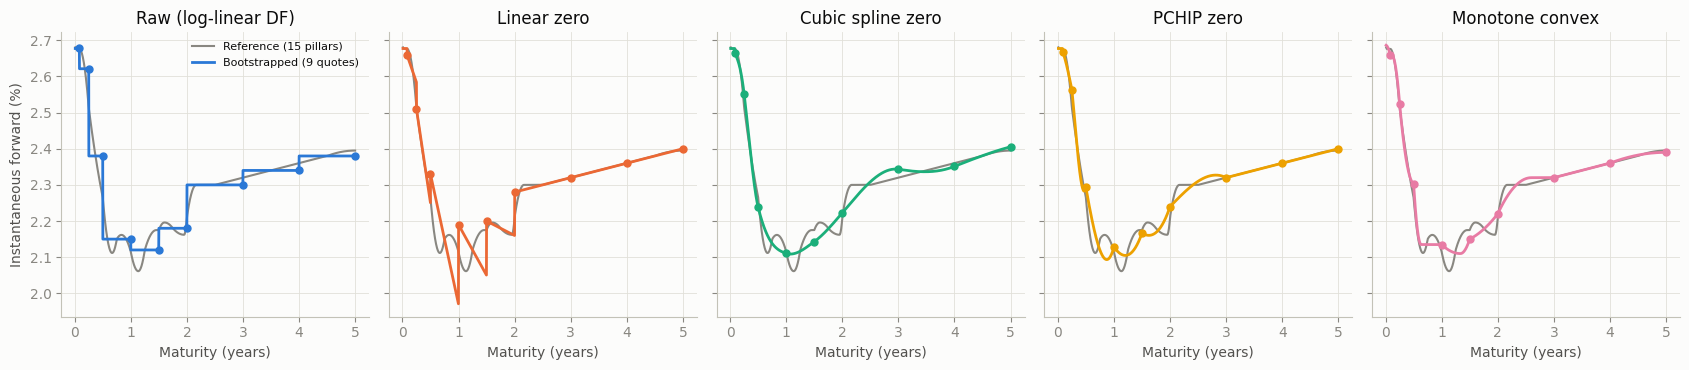
\includegraphics[width=\textwidth]{bootstrap_roundtrip.png}
    \caption{Instantaneous forwards of the curves bootstrapped from 9 quotes (colour) against the 15-pillar reference (grey). Dots: instrument maturities.}
    \label{fig:roundtrip}
\end{figure}

\subsection{Real market data: US Treasury par yields}
\label{sec:treasury}
We now bootstrap the Treasury curve of 21 September 2026 from its 14 quotes, with the conventions of Section~\ref{sec:data}. The three methods tested reprice all the quotes, with maximum residuals of $3.5\times10^{-13}\bp$ (raw, $15$ ms), $2.8\times10^{-13}\bp$ (cubic spline, $71$ ms) and $3.5\times10^{-13}\bp$ (monotone convex, $111$ ms). Table~\ref{tab:treasury} gives the quotes and the bootstrapped zero rates.

\begin{table}[htbp]
\centering
\small
\begin{tabular}{@{}lrrrrrrr@{}}
\toprule
Tenor & 1M & 1.5M & 2M & 3M & 4M & 6M & 1Y \\
Instrument & ZC & ZC & ZC & ZC & ZC & ZC & ZC (s.a.) \\
Quote (\%) & 3.96 & 4.02 & 4.10 & 4.17 & 4.26 & 4.27 & 4.45 \\
Zero rate (\%) & 3.954 & 4.010 & 4.086 & 4.148 & 4.230 & 4.225 & 4.401 \\
\midrule
Tenor & 2Y & 3Y & 5Y & 7Y & 10Y & 20Y & 30Y \\
Instrument & par bond & par bond & par bond & par bond & par bond & par bond & par bond \\
Quote (\%) & 4.76 & 4.82 & 4.83 & 4.89 & 4.96 & 5.33 & 5.29 \\
Zero rate (\%) & 4.713 & 4.771 & 4.778 & 4.844 & 4.923 & 5.402 & 5.271 \\
\bottomrule
\end{tabular}
\caption{US Treasury par yield curve (21/09/2026) and bootstrapped continuously compounded zero rates (monotone convex).}
\label{tab:treasury}
\end{table}

\begin{figure}[htbp]
    \centering
    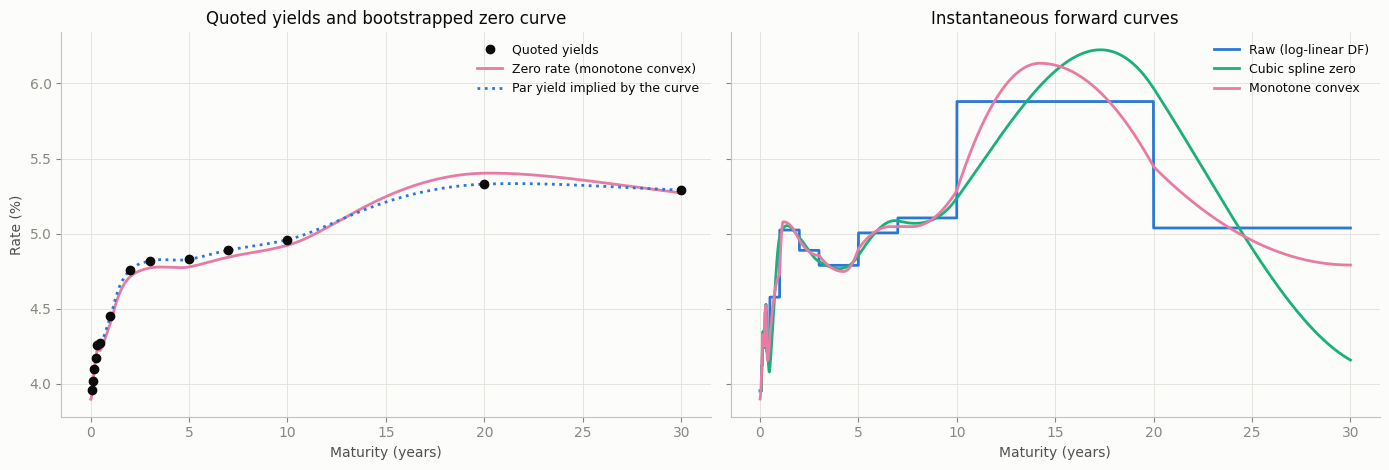
\includegraphics[width=\textwidth]{treasury_curves.png}
    \caption{US Treasury curve of 21/09/2026. Left: quoted yields, bootstrapped zero curve and par yields implied by the curve. Right: instantaneous forward curves of three methods.}
    \label{fig:treasury}
\end{figure}

The par yields implied by the curve go through every quote (Figure~\ref{fig:treasury}, left), but with sparse long-end quotes the forward curves diverge (right):
\begin{itemize}
    \item \textbf{raw}: the forward is $5.88\%$ on $10$--$20$ years and drops by $84\bp$ to $5.04\%$ on $20$--$30$ years;
    \item \textbf{$10$--$20$ years}: the forward at both ends of the segment is below the segment's average $5.88\%$, so by Remark~\ref{rem:mean} every continuous method must rise above it in the middle: monotone convex peaks at $6.1\%$ and the cubic spline at $6.2\%$;
    \item \textbf{beyond $20$ years}: the cubic spline dives to $4.2\%$ at 30 years, below every quote of the curve, while monotone convex stays around $4.8\%$.
\end{itemize}
Long-dated forwards, which drive long-dated exotics such as callable bonds or 30-year Bermudan swaptions, are therefore largely a product of the interpolation choice, by almost $90\bp$ at 30 years between two exact methods (raw $5.04\%$, cubic spline $4.2\%$).

\clearpage
% ===============================================================
\section{Curve History and Principal Components}
\label{sec:pca}
% ===============================================================

\subsection{Method}
The Treasury curve is bootstrapped (monotone convex) on each of the 181 dates of the file, which takes $20.8$ seconds, i.e. about $115$ ms per curve. The zero rates are read on a fixed grid of 10 maturities $(0.25,0.5,1,2,3,5,7,10,20,30)$ years, and the daily changes $\Delta r_t\in\R^{10}$ (in basis points, 180 observations) are decomposed in principal components: with $\Sigma$ the sample covariance matrix of the changes,
\begin{equation}
    \Sigma=\sum_{k=1}^{10}\lambda_k\,e_ke_k^\top,\qquad \lambda_1\ge\dots\ge\lambda_{10}\ge0,
\end{equation}
the eigenvector $e_k$ is the shape of the $k$-th factor and $\lambda_k/\sum_j\lambda_j$ the share of variance it explains. The sign of each eigenvector is chosen so that its average loading is positive.

\subsection{Results}
The first three components explain $79.6\%$, $13.2\%$ and $2.7\%$ of the variance ($95.5\%$ together; the fourth explains $1.4\%$), and have the classical shapes identified by Litterman and Scheinkman~\cite{litterman} (Figure~\ref{fig:pca}):
\begin{itemize}
    \item \textbf{PC1, level}: all loadings positive, with a maximum around 5 years ($0.42$) and a small loading at 3 months ($0.07$). The very short end, anchored by the Fed policy rate, moves less than the belly of the curve;
    \item \textbf{PC2, slope}: positive up to 3 years, zero around 5 years and strongly negative at the long end ($-0.52$ at 30 years): a steepening or flattening of the curve;
    \item \textbf{PC3, curvature}: positive at both ends ($0.64$ at 3 months, $0.34$ at 30 years) and negative in the belly ($-0.25$ at 3 years): a change of the convexity of the curve.
\end{itemize}

\begin{figure}[htbp]
    \centering
    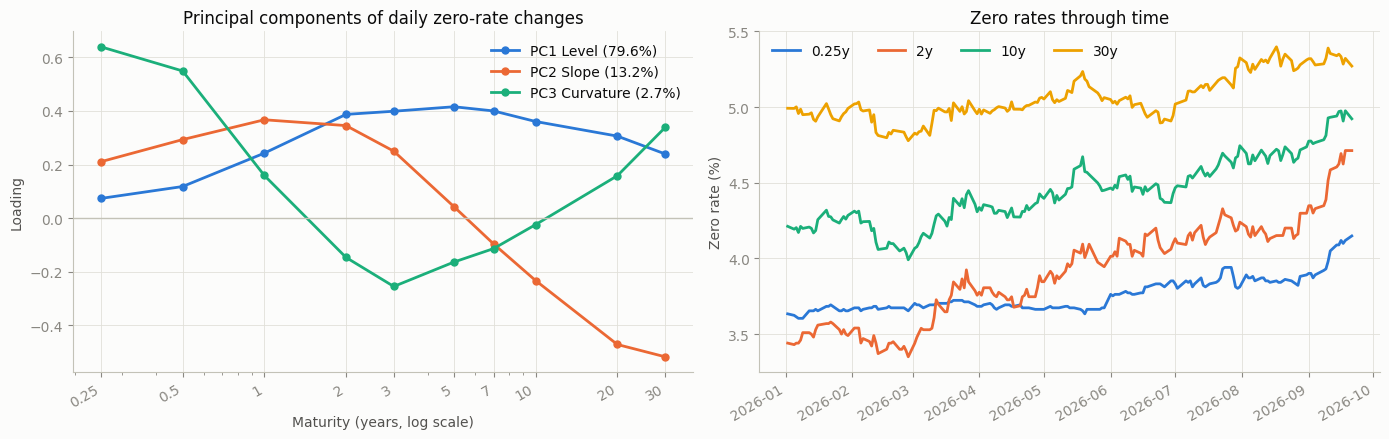
\includegraphics[width=\textwidth]{pca.png}
    \caption{Left: principal components of daily zero-rate changes of the US Treasury curve (2/01/2026 to 21/09/2026). Right: zero rates at 3 months, 2, 10 and 30 years through time.}
    \label{fig:pca}
\end{figure}

Over the period, all the rates rose, the 2-year by more than $120\bp$ (from $3.4\%$ to $4.7\%$) and the 30-year by about $30\bp$, so that the curve flattened between 2 and 30 years. Three factors are enough to describe almost all the daily moves of the curve: this is the empirical justification of the parsimonious factor models (Nelson--Siegel factors, two- and three-factor short-rate models), and a one-factor model such as Hull--White, which essentially captures the level, misses about $20\%$ of the variance and, more importantly, the decorrelation between short and long rates.

\clearpage
% ===============================================================
\section{Risk: Key-Rate Sensitivities of an Off-Pillar Cash Flow}
\label{sec:risk}
% ===============================================================

\subsection{Setting}
A zero-coupon bond of notional $N=1{,}000{,}000\,\eur$ maturing at $T=3.5$ years, between the 3- and 4-year swap pillars, is priced on the curve bootstrapped from the 9 EURIBOR quotes of Table~\ref{tab:quotes}. Each quote is bumped by $+1\bp$ in turn, the curve is re-bootstrapped and the bond repriced:
\begin{equation}
    \mathrm{KR}_k=N\Bigl(P^{(q+\epsilon e_k)}(0,T)-P^{(q)}(0,T)\Bigr),\qquad \epsilon=1\bp.
\end{equation}
$\mathrm{KR}_k$ is the bond's sensitivity to the $k$-th hedging instrument: the hedge is obtained by selling $\mathrm{KR}_k/\mathrm{DV01}_k$ of instrument $k$. The interpolation therefore decides which instruments hedge the bond. We also compute the parallel sensitivity (all quotes bumped together).

\subsection{Results}

\begin{table}[htbp]
\centering
\small
\setlength{\tabcolsep}{4pt}
\begin{tabular}{@{}lrrrrrrrrrrr@{}}
\toprule
Method & D1M & D3M & D6M & FRA & S1.5y & S2y & S3y & S4y & S5y & Sum & Parallel \\
\midrule
Raw & 0.00 & 0.00 & 1.05 & 1.05 & 0.00 & 4.19 & $-135.35$ & $-186.94$ & 0.00 & $-315.99$ & $-315.93$ \\
Linear zero & 0.00 & 0.00 & 1.07 & 1.07 & 0.00 & 4.28 & $-158.84$ & $-163.58$ & 0.00 & $-316.01$ & $-315.94$ \\
Cubic spline & $-0.43$ & 1.67 & 2.11 & 5.07 & $-30.02$ & 63.92 & $-197.98$ & $-184.78$ & 24.20 & $-316.23$ & $-316.17$ \\
PCHIP & 0.00 & 0.00 & 1.04 & 1.04 & 0.00 & 31.43 & $-165.38$ & $-201.46$ & 16.48 & $-316.84$ & $-315.94$ \\
Mon. convex & 0.00 & 0.00 & 1.05 & 1.05 & 0.00 & 15.87 & $-186.33$ & $-238.83$ & 28.99 & $-378.22$ & $-315.94$ \\
\bottomrule
\end{tabular}
\caption{Sensitivity (\eur) of a $1{,}000{,}000\,\eur$ zero-coupon bond maturing in 3.5 years to a $+1\bp$ bump of each quote, and to a parallel $+1\bp$ bump of all quotes.}
\label{tab:krd}
\end{table}

The parallel sensitivity is the same for every method, $-316\,\eur$ per basis point (Table~\ref{tab:krd}). It is close to the zero-rate DV01 $N\,T\,P(0,T)\times10^{-4}\approx323\,\eur$, and slightly smaller because a parallel $1\bp$ bump of the par rates moves the 3.5-year zero rate by slightly less than $1\bp$. Its split across instruments, however, depends on the method:
\begin{itemize}
    \item \textbf{raw and linear zero}: the bond is hedged by the 3- and 4-year swaps only, plus a small annuity effect on the shorter instruments (whose bumps move the discount factors of the swap coupons). For raw, $y(3.5)=\frac12\bigl(y(3)+y(4)\bigr)$, so the split between the two swaps is close to the ratio $3:4$ of the zero-rate sensitivities, $N P(0,T)\cdot\frac{t_i}{2}\times10^{-4}=139$ and $185\,\eur$;
    \item \textbf{cubic spline}: part of the risk leaks onto the 1.5-, 2- and 5-year swaps, with alternating signs ($-30$, $+64$, $+24\,\eur$): a 3.5-year cash flow would be hedged with 1.5-year swaps;
    \item \textbf{PCHIP and monotone convex}: the risk spreads to the neighbouring 2- and 5-year swaps, as expected from their almost-local construction;
    \item \textbf{monotone convex}: the key rates \emph{do not add up} to the parallel sensitivity ($-378$ against $-316\,\eur$), and PCHIP is slightly off too ($-317$).
\end{itemize}

\subsection{Non-linearity of the monotone convex method}
The last point is not a numerical error. Between 2 and 5 years the EURIBOR rates increase by exactly $2\bp$ a year, so the discrete forwards increase regularly by $2\bp$ per segment and the corrections $g_0,g_1$ of~\eqref{eq:mc-g} are tiny, about $1$--$2\bp$. A $1\bp$ bump of a swap quote moves the neighbouring discrete forwards by several basis points, i.e. by more than $g_0,g_1$, and pushes them across the boundaries of the Hagan--West regions of Table~\ref{tab:mc-regions}. The curve stays continuous in its inputs but becomes strongly non-linear, and the sensitivity depends on the size and sign of the bump (Table~\ref{tab:bumpsize}).

\begin{table}[htbp]
\centering
\small
\begin{tabular}{@{}llrrrr@{}}
\toprule
Method & Quote bumped & $+1\bp$ & $+0.1\bp$ & $-0.1\bp$ & $-1\bp$ \\
\midrule
\multirow{2}{*}{Raw} & Swap 3y & $-135.35$ & $-135.35$ & $-135.35$ & $-135.35$ \\
 & Swap 4y & $-186.94$ & $-186.94$ & $-186.94$ & $-186.94$ \\
\midrule
\multirow{2}{*}{PCHIP} & Swap 3y & $-165.38$ & $-177.47$ & $-180.53$ & $-195.27$ \\
 & Swap 4y & $-201.46$ & $-186.01$ & $-182.83$ & $-170.35$ \\
\midrule
\multirow{2}{*}{Monotone convex} & Swap 3y & $-186.33$ & $-152.68$ & $-152.68$ & $-110.68$ \\
 & Swap 4y & $-238.83$ & $-210.86$ & $-210.86$ & $-140.57$ \\
\bottomrule
\end{tabular}
\caption{Bond sensitivity per basis point (\eur) for different bump sizes of the 3- and 4-year swap quotes.}
\label{tab:bumpsize}
\end{table}

With raw interpolation the sensitivity per basis point is identical whatever the bump: the curve is linear in the pillar values $y_i$, and the remaining non-linearity of the par-rate equations is invisible at this scale. PCHIP is mildly non-linear ($-165$ to $-195\,\eur$ per bp on the 3-year swap) since its node slopes are harmonic means of the neighbouring ones. Monotone convex is strongly so: $-111$ to $-186\,\eur$ on the 3-year swap and $-141$ to $-239\,\eur$ on the 4-year swap. For small bumps ($\pm0.1\bp$) the two one-sided sensitivities agree, so the curve is locally differentiable; the non-linearity appears when the bump crosses a region boundary, which happens here between $0.1$ and $1\bp$.

For hedging this is a real drawback: key-rate risks must then be computed with a documented bump size (or a parallel bump), and a local and linear method such as raw may be preferred for the risk engine. More generally, \emph{a hedge computed with one interpolation is not a hedge under another}: the method must be fixed once for both pricing and risk.

\clearpage
% ===============================================================
\section{Using the Curve Downstream}
\label{sec:downstream}
% ===============================================================

\subsection{The \texttt{YieldCurve} class}
\texttt{YieldCurve} gathers what pricing models need. It is built from zero rates in any compounding, from discount factors, or by the \texttt{Bootstrapper}, and it is callable: \texttt{curve(T)} returns the continuously compounded zero rate, so it can be passed directly as the \texttt{zc\_rate} argument of \texttt{ForwardCurve}, \texttt{BlackScholes} or \texttt{HestonModel}. Table~\ref{tab:downstream} lists its main outputs on the monotone convex EURIBOR curve.

\begin{table}[htbp]
\centering
\small
\begin{tabular}{@{}lll@{}}
\toprule
Quantity & Method & Value \\
\midrule
Zero rate $r(2)$, continuous / annual & \texttt{curve(2.0)}, \texttt{zero\_rate(2.0, 1)} & $2.2400\%$ / $2.2653\%$ \\
Discount factor $P(0,2)$ & \texttt{discount(2.0)} & $0.956189$ \\
Simple forward $1\text{y}\times1.5\text{y}$ (FRA) & \texttt{forward\_rate(1, 1.5, 'simple')} & $2.1313\%$ \\
Instantaneous forward $f(0,2)$ & \texttt{instantaneous\_forward(2.0)} & $2.2100\%$ \\
5-year annual par swap rate & \texttt{par\_rate(5.0, 1)} & $2.3253\%$ \\
Monte Carlo drift $\int_1^{1.5}f(0,s)\,\dd s$ & \texttt{integrated\_short\_rate(1, 1.5)} & $0.010600$ \\
Parallel $+10\bp$ scenario, $r(2)$ & \texttt{shifted(10)(2.0)} & $2.3400\%$ \\
Key-rate bump of pillar $i$ & \texttt{bumped(i, bp)} & -- \\
\bottomrule
\end{tabular}
\caption{Main outputs of \texttt{YieldCurve} (monotone convex EURIBOR curve). All methods are vectorized in $T$.}
\label{tab:downstream}
\end{table}

The method \texttt{integrated\_short\_rate} returns $y(t_2)-y(t_1)=\ln\bigl(P(0,t_1)/P(0,t_2)\bigr)$, the deterministic drift of the log-spot over a Monte Carlo step: it is exact for any time step, whatever the interpolation, because it is computed from $y$ and not by integrating $f$ numerically.

\subsection{Equity models}
In the Heston and LSV papers, the rate curve only enters through $D(T)=P(0,T)$ and the forward $F(T)$. Over the option maturities (9 days to 5 years) the exact interpolations differ by less than a basis point on the zero rates (Section~\ref{sec:comparison}), i.e. less than $0.05\%$ on a 5-year discount factor, which is negligible compared with the uncertainty on the implied dividend curve. The choice of the interpolation is a second-order question for equity derivatives.

\subsection{Short-rate models}
It is a first-order question for rate models. The one-factor Hull--White model implemented in \texttt{hull\_white\_1F.py},
\begin{equation}
    \dd r_t=\bigl(\vartheta(t)-ar_t\bigr)\dd t+\sigma\,\dd W_t,
\end{equation}
is fitted exactly to the initial curve by writing $r_t=x_t+\alpha(t)$, with $\dd x_t=-ax_t\,\dd t+\sigma\,\dd W_t$, $x_0=0$, and
\begin{equation}
    \alpha(t)=f(0,t)+\frac{\sigma^2}{2a^2}\bigl(1-e^{-at}\bigr)^2,
    \qquad
    \vartheta(t)=\frac{\partial f(0,t)}{\partial t}+af(0,t)+\frac{\sigma^2}{2a}\bigl(1-e^{-2at}\bigr)
\end{equation}
(Brigo and Mercurio~\cite{brigomercurio}, Chapter 3). The expected short rate path is thus essentially the instantaneous forward curve: with raw interpolation it is a step function and $\vartheta(t)$ contains Dirac masses at the pillars; with a natural cubic spline on the Treasury curve, it inherits the $6.2\%$ hump and the dive to $4.2\%$ at 30 years. The implementation avoids differentiating $f$: bond prices use $P(0,T)/P(0,t)$ and the Monte Carlo uses $\int_0^t\alpha(s)\,\dd s=y(t)+\frac{\sigma^2}{2a^2}\int_0^t(1-e^{-as})^2\,\dd s$ in closed form. The forward shape nevertheless drives the distribution of future rates, hence the value of path-dependent and callable products. A continuous forward curve such as monotone convex is the natural input.

\clearpage
% ===============================================================
\section{Limitations}
\label{sec:limits}
% ===============================================================

\paragraph{Single-curve framework.} The same curve discounts the cash flows and projects the floating rates. Since 2008 the market uses an OIS curve (\texteuro STR, SOFR) for discounting collateralized trades, and a separate projection curve for each tenor (EURIBOR 3M, 6M), the basis spreads between them being material~\cite{ametrano}. The floating leg of a swap is then no longer worth $1-P(0,T)$, and~\eqref{eq:par} does not hold.

\paragraph{Conventions.} Times are plain year fractions: no day-count conventions (ACT/360 for deposits, 30/360 for fixed legs), business-day calendars, settlement lags or payment delays. Quotes are therefore not exactly comparable with market screens, and the error is of the order of a few basis points on short-dated instruments.

\paragraph{Data.} The EURIBOR data are assumed to be continuously compounded zero rates rounded to the basis point; this rounding alone creates up to $9.5\bp$ of noise on the discrete forwards. The Treasury bills are treated with a simplified convention (their yields are bond-equivalent yields on a discount basis), and Treasury coupon yields contain liquidity and on-the-run effects that a smooth curve should not reproduce exactly.

\paragraph{Instruments.} No futures among the instruments, and therefore no convexity adjustment; no turn-of-year effect on the short end; no basis swaps.

\paragraph{Monotone convex.} The positivity collar of Hagan and West is not implemented, and the method is strongly non-linear when consecutive discrete forwards are close, which makes key-rate risks depend on the bump size (Section~\ref{sec:risk}).

\paragraph{Risk.} Sensitivities are computed by full re-bootstrap with finite bumps, which costs one bootstrap per instrument and is subject to the non-linearity above. The bootstrap Jacobian is not used.

% ===============================================================
\section{Next Steps}
\label{sec:next-steps}
% ===============================================================

\begin{itemize}
    \item Implement a multi-curve bootstrap: \texteuro STR OIS discounting, EURIBOR 3M and 6M projection curves, basis swaps, with the projection curves bootstrapped given the discount curve.
    \item Add day-count conventions, calendars and settlement lags, and futures with a convexity adjustment computed from the Hull--White model.
    \item Compute key-rate risks with the implicit function theorem: since $R(z,q)=0$, $\partial z/\partial q=-(\partial_zR)^{-1}\partial_qR$, which gives all the sensitivities from one Jacobian, and compare them with the finite bumps of Section~\ref{sec:risk} for the non-linear methods.
    \item Implement the positivity collar of the monotone convex method, and compare with tension splines or smoothing splines, which trade exactness for a smoother forward curve.
    \item Use the principal components of Section~\ref{sec:pca} to calibrate the correlation of a two-factor Hull--White (G2++) model, whose file \texttt{hull\_white\_2F.py} is still empty.
    \item Measure the model risk of the interpolation on exotic rate products: price long-dated Bermudan swaptions and callable range accruals with Hull--White on the raw, cubic spline and monotone convex Treasury curves.
\end{itemize}

% ===============================================================
\section{Conclusion}
\label{sec:conclusion}
% ===============================================================

The construction of a yield curve looks like a solved problem, since every exact interpolation reprices the market instruments to machine precision. This paper shows that what is left free by the market, the curve between the pillars, matters. The interpolation must be judged on the instantaneous forward curve and not on the zero curve: on the EURIBOR 6M curve, methods that agree within a basis point on zero rates produce step, saw-tooth or oscillating forwards. Monotone convex is the best compromise for pricing: exact at the pillars, continuous forward, local, and with the lowest forward variation among the continuous methods. The raw method remains the simplest, local and linear choice, well suited to a risk engine, at the cost of a step forward curve. Natural cubic splines are smooth but non-local and overshoot at the long end; they should not be used for risk. The parametric Nelson--Siegel and Svensson curves are good descriptive tools but do not reprice the inputs.

The bootstrap reprices the instruments exactly with any exact interpolation, through a sequential solve for raw interpolation and a simultaneous solve for the non-local methods. But a round trip from 9 quotes recovers the reference curve only within $1$--$3\bp$ on zero rates, and on the real US Treasury curve the 30-year forward differs by more than $60\bp$ between monotone convex and the cubic spline. The principal components of 181 bootstrapped Treasury curves recover the level, slope and curvature factors, which explain $95.5\%$ of the daily moves.

Finally, the interpolation determines the hedge of a cash flow that does not fall on a pillar: the parallel risk of a 3.5-year bond is the same under every method, but its split across instruments is not, and the strong non-linearity of the monotone convex method makes its key rates depend on the bump size. A curve is therefore not only a set of numbers but a modelling choice, which must be fixed once for pricing and risk, and documented.

\clearpage

% ===============================================================
\appendix
\section{Python Implementation (Excerpts)}
\label{app:code}
% ===============================================================

The following listings are excerpts of the implementation (package \texttt{Fixed\_Income\_Models}), slightly simplified (sanity checks and printing removed). The full scripts and the notebook \texttt{yield\_curve.ipynb} are available on GitHub.

\subsection{Monotone convex node forwards and integrated forward (\texttt{interpolation.py})}
\begin{lstlisting}[style=pystyle]
def _fit(self):
    tau = np.concatenate([[0.0], self.t])
    yt = np.concatenate([[0.0], self.yt])
    fd = np.diff(yt) / np.diff(tau)        # discrete forwards on (tau_{i-1}, tau_i]
    n = len(fd)
    f = np.empty(n + 1)                    # instantaneous forwards at the nodes
    for i in range(1, n):
        w = (tau[i] - tau[i - 1]) / (tau[i + 1] - tau[i - 1])
        f[i] = w * fd[i] + (1 - w) * fd[i - 1]
    f[0] = fd[0] - 0.5 * (f[1] - fd[0])
    f[n] = fd[n - 1] - 0.5 * (f[n - 1] - fd[n - 1])
    self._tau, self._ytau, self._fd, self._fnode = tau, yt, fd, f

def _y_inner(self, T):
    i, h, g, G = self._gG(T)               # segment, length, correction g and its integral G
    return self._ytau[i] + (T - self._tau[i]) * self._fd[i] + h * G

def _f_inner(self, T):
    i, h, g, G = self._gG(T)
    return self._fd[i] + g
\end{lstlisting}

\subsection{Instruments (\texttt{instruments.py}) and par rate (\texttt{yield\_curve.py})}
\begin{lstlisting}[style=pystyle]
class Deposit(Instrument):
    def implied_quote(self, curve):
        return (1.0 / curve.discount(self.maturity) - 1.0) / self.maturity

class FRA(Instrument):
    def implied_quote(self, curve):
        return curve.forward_rate(self.start, self.maturity, compounding='simple')

class Swap(Instrument):
    def implied_quote(self, curve):
        return curve.par_rate(self.maturity, self.frequency)

# YieldCurve
def annuity(self, maturity, frequency=1):
    times = self.schedule(maturity, frequency)
    deltas = np.diff(np.concatenate([[0.0], times]))
    return float(np.sum(deltas * self.discount(times)))

def par_rate(self, maturity, frequency=1):
    return (1.0 - self.discount(maturity)) / self.annuity(maturity, frequency)
\end{lstlisting}

\subsection{Bootstrap (\texttt{bootstrap.py})}
\begin{lstlisting}[style=pystyle]
def _sequential(self):
    """ Pillar-by-pillar bootstrap with raw interpolation. """
    z = np.zeros(len(self.instruments))
    for i, inst in enumerate(self.instruments):
        def f(x):
            z[i] = x
            return inst.residual(YieldCurve(self.times[:i + 1], z[:i + 1], 'raw'))
        z[i] = brentq(f, -0.5, 1.0, xtol=1e-15, rtol=1e-15, maxiter=500)
    return z

def run(self):
    z = self._sequential()
    if INTERPOLATORS[self.method] is not INTERPOLATORS['raw']:
        # non-local method : all the equations together, from the raw solution
        z = root(self._residuals, z, method='hybr', tol=1e-15).x
    self.curve = YieldCurve(self.times, z, self.method)
    self.max_residual_bp = 1e4 * float(np.max(np.abs(self._residuals(z))))
    return self.curve
\end{lstlisting}

\subsection{Key-rate sensitivities (notebook)}
\begin{lstlisting}[style=pystyle]
def bond_value(method, bumps_bp=None):
    # Value of the bond on the curve bootstrapped from the quotes shifted by bumps_bp
    bumped_quotes = copy.deepcopy(quotes)
    for q, bp in zip(bumped_quotes, bumps_bp if bumps_bp is not None else [0.0] * len(quotes)):
        q.quote += bp * 1e-4
    return notional * Bootstrapper(bumped_quotes, method=method).run().discount(maturity)

base = bond_value(m)
key_rates = [bond_value(m, np.eye(len(quotes))[k]) - base for k in range(len(quotes))]
parallel = bond_value(m, np.ones(len(quotes))) - base
\end{lstlisting}

\section{Notation}
\label{app:notation}

\begin{table}[h]
\centering
\begin{tabular}{@{}lp{11.5cm}@{}}
\toprule
Symbol & Meaning \\
\midrule
$P(0,T)$ & Zero-coupon bond price (discount factor) for maturity $T$ \\
$y(T)=-\ln P(0,T)$ & Integrated forward \\
$r(T)=y(T)/T$ & Continuously compounded zero rate \\
$f(0,T)=y'(T)$ & Instantaneous forward rate \\
$f(0;T_1,T_2),\ F(0;T_1,T_2)$ & Continuous and simple forward rates between $T_1$ and $T_2$ \\
$t_i,\ r_i,\ \tau_i$ & Pillar times, pillar zero rates, nodes including the origin $\tau_0=0$ \\
$f^d_i$ & Discrete forward on $(t_{i-1},t_i]$ \\
$f_i,\ g_0,\ g_1,\ g(x)$ & Monotone convex node forwards and correction function \\
$\beta_k,\ \lambda_k$ & Nelson--Siegel / Svensson coefficients and time scales \\
$A(T),\ S(T)$ & Annuity and par swap rate \\
$q_k,\ \hat q_k,\ R_k$ & Market quote, quote implied by the curve and residual of instrument $k$ \\
$z$ & Vector of the zero rates at the pillars (bootstrap unknowns) \\
$\Sigma,\ \lambda_k,\ e_k$ & Covariance of daily zero-rate changes, its eigenvalues and eigenvectors \\
$\mathrm{KR}_k$ & Key-rate sensitivity to instrument $k$ \\
$a,\ \sigma,\ \alpha(t),\ \vartheta(t)$ & Hull--White mean reversion, volatility, deterministic shift and drift \\
\bottomrule
\end{tabular}
\caption{Main notation.}
\label{tab:notation}
\end{table}

\clearpage

% ===============================================================
\begin{thebibliography}{99}
% ===============================================================

\bibitem{haganwest2006}
P. S. Hagan and G. West,
\textit{Interpolation methods for curve construction},
Applied Mathematical Finance, 13(2):89--129, 2006.

\bibitem{haganwest2008}
P. S. Hagan and G. West,
\textit{Methods for constructing a yield curve},
Wilmott Magazine, May 2008, 70--81.

\bibitem{nelsonsiegel}
C. R. Nelson and A. F. Siegel,
\textit{Parsimonious modeling of yield curves},
Journal of Business, 60(4):473--489, 1987.

\bibitem{svensson}
L. E. O. Svensson,
\textit{Estimating and interpreting forward interest rates: Sweden 1992--1994},
NBER Working Paper 4871, 1994.

\bibitem{fritsch}
F. N. Fritsch and R. E. Carlson,
\textit{Monotone piecewise cubic interpolation},
SIAM Journal on Numerical Analysis, 17(2):238--246, 1980.

\bibitem{brent}
R. P. Brent,
\textit{Algorithms for Minimization without Derivatives},
Prentice-Hall, 1973.

\bibitem{powell}
M. J. D. Powell,
\textit{A hybrid method for nonlinear equations},
in P. Rabinowitz (ed.), Numerical Methods for Nonlinear Algebraic Equations, Gordon and Breach, 1970, 87--114.

\bibitem{litterman}
R. Litterman and J. Scheinkman,
\textit{Common factors affecting bond returns},
Journal of Fixed Income, 1(1):54--61, 1991.

\bibitem{brigomercurio}
D. Brigo and F. Mercurio,
\textit{Interest Rate Models -- Theory and Practice},
2nd edition, Springer Finance, 2006.

\bibitem{hullwhite}
J. Hull and A. White,
\textit{Pricing interest-rate-derivative securities},
Review of Financial Studies, 3(4):573--592, 1990.

\bibitem{ametrano}
F. M. Ametrano and M. Bianchetti,
\textit{Everything you always wanted to know about multiple interest rate curve bootstrapping but were afraid to ask},
SSRN Working Paper 2219548, 2013.

\bibitem{andersenpiterbarg}
L. B. G. Andersen and V. V. Piterbarg,
\textit{Interest Rate Modeling, Volume I: Foundations and Vanilla Models},
Atlantic Financial Press, 2010.

\bibitem{data}
\textit{Equity implied volatility surface -- market data},
Available at: \url{https://github.com/Idriss-Afra/Equity-Implied-Volatility-Surface/tree/main/MarketData}

\bibitem{treasury}
U.S. Department of the Treasury,
\textit{Daily Treasury Par Yield Curve Rates},
Available at: \url{https://home.treasury.gov/resource-center/data-chart-center/interest-rates}

\end{thebibliography}

\end{document}
